\begin{figure}[ht]
\centering
    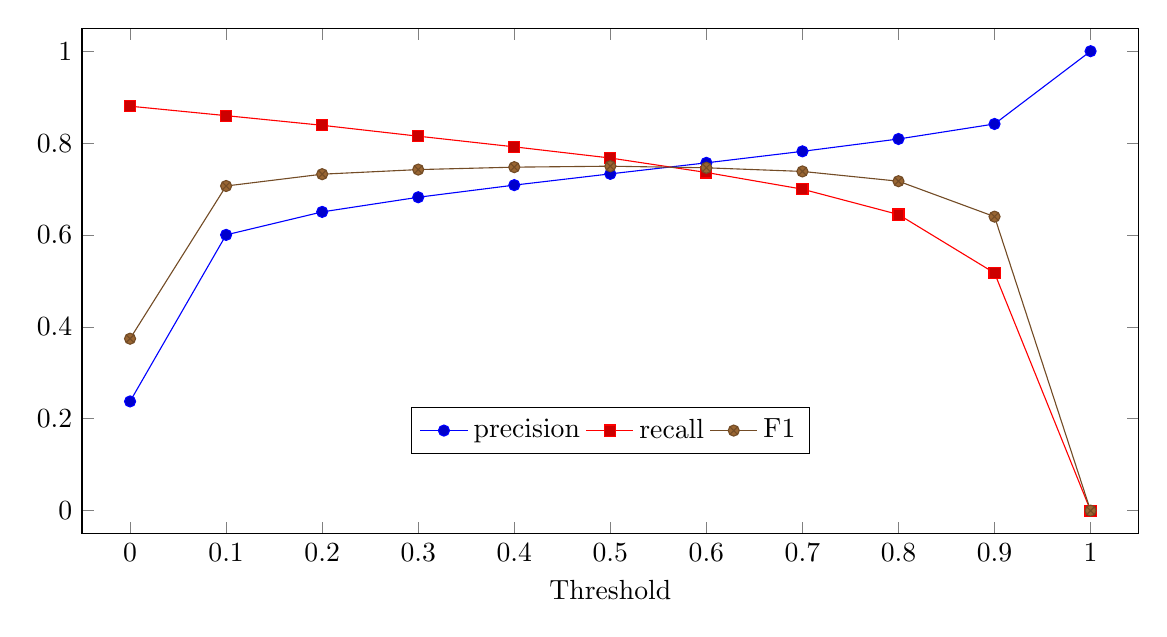
\begin{tikzpicture}
        \begin{axis}[
                height=8cm,
                width=15cm,
                xlabel=Threshold,
                legend style={at={(0.5,0.25)},
                anchor=north,legend columns=-1},
                enlarge x limits=0.05,
                enlarge y limits=0.05,
            ]
            \addplot+[sharp plot] coordinates
            {
                (0.0,0.2377)
                (0.1,0.6002)
                (0.2,0.6502) 
                (0.3,0.6821) 
                (0.4,0.7085) 
                (0.5,0.7330)
                (0.6,0.7570) 
                (0.7,0.7820) 
                (0.8,0.8089) 
                (0.9,0.8416) 
                (1.0,1.0000)};

            \addplot+[sharp plot] coordinates
            {
                (0.0,0.8803)
                (0.1,0.8597) 
                (0.2,0.8387) 
                (0.3,0.8150) 
                (0.4,0.7918) 
                (0.5,0.7675)
                (0.6,0.7360) 
                (0.7,0.6997) 
                (0.8,0.6445) 
                (0.9,0.5172) 
                (1.0,0.0000)};

            \addplot+[sharp plot] coordinates
            {
                (0.0,0.3742)
                (0.1,0.7066) 
                (0.2,0.7323) 
                (0.3,0.7423) 
                (0.4,0.7476) 
                (0.5,0.7497)
                (0.6,0.7462) 
                (0.7,0.7383) 
                (0.8,0.7170) 
                (0.9,0.6399) 
                (1.0,0.0000)};

            \legend{precision,recall,F1}
        \end{axis}
    \end{tikzpicture}
\caption{\label{i:classify-threshold} Performance for the pipeline system
with different thresholds. }
\end{figure}
